%%%%%%%%%%%%%%%%%%%%%%%%%%%%%%%%%%%%%%%%%
% Beamer Presentation
% LaTeX Template
% Version 1.0 (10/11/12)
%
% This template has been downloaded from:
% http://www.LaTeXTemplates.com
%
% License:
% CC BY-NC-SA 3.0 (http://creativecommons.org/licenses/by-nc-sa/3.0/)
%
%%%%%%%%%%%%%%%%%%%%%%%%%%%%%%%%%%%%%%%%%

%----------------------------------------------------------------------------------------
%	PACKAGES AND THEMES
%----------------------------------------------------------------------------------------


\documentclass{beamer}
\usepackage[utf8]{inputenc} % Für Umlaute unter Linux
\definecolor{TUGreen}{HTML}{84b819} % TU-Grün definieren
\mode<presentation> {

% The Beamer class comes with a number of default slide themes
% which change the colors and layouts of slides. Below this is a list
% of all the themes, uncomment each in turn to see what they look like.

%\usetheme{default}
%\usetheme{AnnArbor}
%\usetheme{Antibes}
%\usetheme{Bergen}
%\usetheme{Berkeley}
%\usetheme{Berlin}
%\usetheme{Boadilla}
%\usetheme{CambridgeUS}
%\usetheme{Copenhagen}
%\usetheme{Darmstadt}
%\usetheme{Dresden}
%\usetheme{Frankfurt}
%\usetheme{Goettingen}
%\usetheme{Hannover}
%\usetheme{Ilmenau}
%\usetheme{JuanLesPins}
%\usetheme{Luebeck}
\usetheme{Madrid}
%\usetheme{Malmoe}
%\usetheme{Marburg}
%\usetheme{Montpellier}
%\usetheme{PaloAlto}
%\usetheme{Pittsburgh}
%\usetheme{Rochester}
%\usetheme{Singapore}
%\usetheme{Szeged}
%\usetheme{Warsaw}

% As well as themes, the Beamer class has a number of color themes
% for any slide theme. Uncomment each of these in turn to see how it
% changes the colors of your current slide theme.

%\usecolortheme{albatross}
%\usecolortheme{beaver}
%\usecolortheme{beetle}
%\usecolortheme{crane}
%\usecolortheme{dolphin}
%\usecolortheme{dove}
%\usecolortheme{fly}
%\usecolortheme{lily}
%\usecolortheme{orchid}
%\usecolortheme{rose}
%\usecolortheme{seagull}
%\usecolortheme{seahorse}
%\usecolortheme{whale}
%\usecolortheme{wolverine}

%\setbeamertemplate{footline} % To remove the footer line in all slides uncomment this line
%\setbeamertemplate{footline}[page number] % To replace the footer line in all slides with a simple slide count uncomment this line

%\setbeamertemplate{navigation symbols}{} % To remove the navigation symbols from the bottom of all slides uncomment this line
\setbeamercolor{structure}{fg=TUGreen!90!black}
}

\usepackage{graphicx} % Allows including images
\usepackage{booktabs} % Allows the use of \toprule, \midrule and \bottomrule in tables
\usepackage{amsmath}
\usepackage{listings}
\usepackage{pgf, tikz} % fuer Graphen
\usepackage[ngerman]{babel}
\usetikzlibrary{shapes,arrows} % fuer Graphen Elemente
\usepackage{csquotes}
\usepackage{url}
% Declare arg max
\DeclareMathOperator*{\argmax}{arg\,max}
\usepackage{dirtytalk}
%----------------------------------------------------------------------------------------
%	TITLE PAGE
%----------------------------------------------------------------------------------------

\title[N-Version Programmierung]{N-Version Programmierung} % The short title appears at the bottom of every slide, the full title is only on the title page

\author{Maximilian Stach} % Your name
\institute[TU Dortmund] % Your institution as it will appear on the bottom of every slide, may be shorthand to save space
{
Technische Universität Dortmund \\ % Your institution for the title page
\medskip
%\textit{blubla@tu-dortmund.de} % Your email address
}
\date{14.02.2017} % Date, can be changed to a custom date

\begin{document}

\begin{frame}
\titlepage % Print the title page as the first slide
\end{frame}

\begin{frame}
\frametitle{Überblick} % Table of contents slide, comment this block out to remove it
\tableofcontents % Throughout your presentation, if you choose to use \section{} and \subsection{} commands, these will automatically be printed on this slide as an overview of your presentation
\end{frame}

%----------------------------------------------------------------------------------------
%	PRESENTATION SLIDES
%----------------------------------------------------------------------------------------

\section{Einleitung}
\subsection{Motivation}
%
%
\begin{frame}
	\frametitle{Überblick}
	\tableofcontents[currentsubsection]
\end{frame}
%
%
\begin{frame}
		\frametitle{Motivation - Kleine und große Katastrophen (1)}
	\begin{columns}
		\begin{column}{0.48\textwidth}
			\begin{figure}
				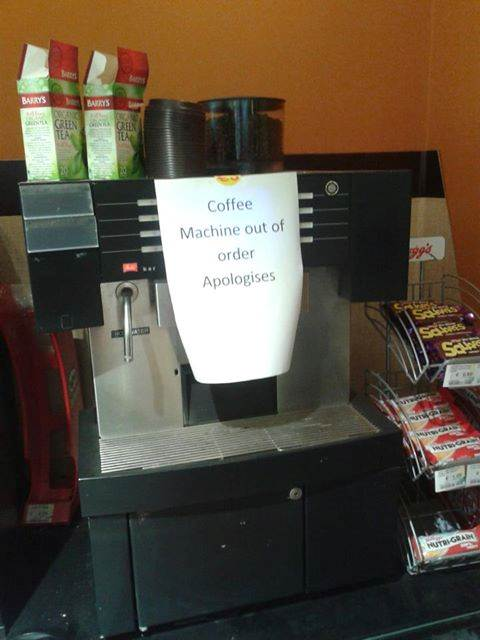
\includegraphics[scale=0.36]{grafiken/broken2}		
				\caption{Defekte Kaffeemaschine
					\footnotemark	
				}		
			\end{figure}
		\end{column}
		\begin{column}{0.48\textwidth}
			Kleine Katastrophe:
			\begin{itemize}
				\item Kaffeemaschine defekt
				\item Folge: Müder Informatiker
			\end{itemize}
		\end{column}		
	\end{columns}
	\footnotetext{Quelle: \url{https://jlonerga.wordpress.com}}
\end{frame}
%
%
\begin{frame}
	\frametitle{Motivation -  Kleine und große Katastrophen (2)}
	\begin{columns}
		\begin{column}{0.48\textwidth}
			\begin{figure}
				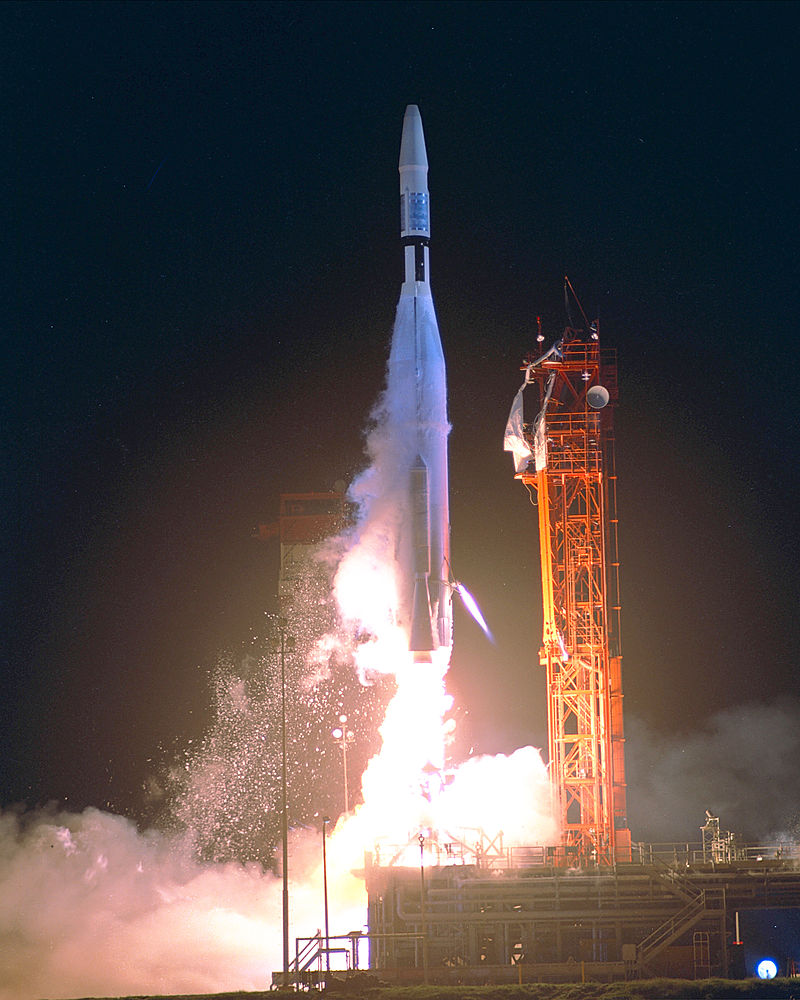
\includegraphics[scale=0.6]{grafiken/mariner}		
				\caption{Fehlerhafte Trägerrakete
					\footnotemark		
				}		
			\end{figure}
		\end{column}
		\begin{column}{0.48\textwidth}
			Große Katastrophe:
			\begin{itemize}
				\item Start der Trägerrakete der Raumsonde \emph{Mariner 1} (1962)
				\pause
				\item Missverständnis beim Implementieren der Spezifikation
				\pause
				\item Folgen:
				\begin{itemize}
					\item Rohe- anstatt geglättete Messdaten
					\item Starke Abweichung vom Kurs
					\item Notsprengung der Rakete nach ca. 5 Minuten
					\item Schaden von ca. 18,5 Millionen Dollar
				\end{itemize}
			\end{itemize}
		\end{column}
		
	\end{columns}
	\footnotetext{Quelle: \url{NASA}}
\end{frame}
%
%
%
\begin{frame}
	\frametitle{Motivation - Lösung für kleine Katastrophen}
	\begin{figure}
		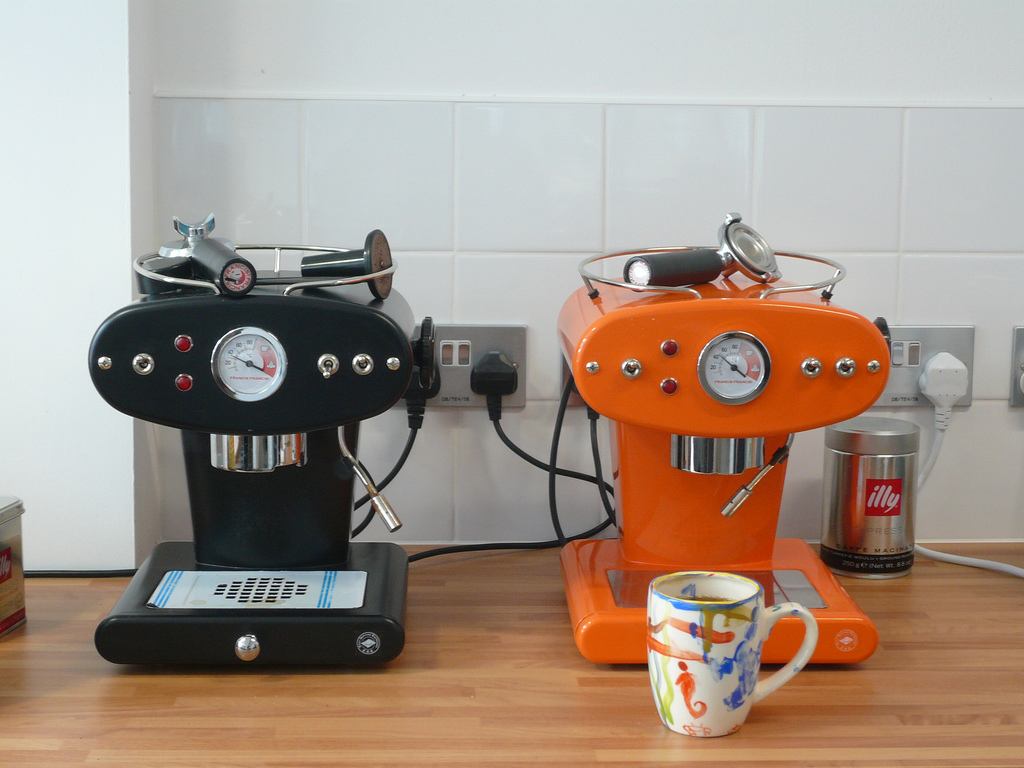
\includegraphics[scale=0.2]{grafiken/working}		
		\caption{Ansatz - Doppelt hält besser
			\footnote{\tiny Quelle: \url{http://www.sarahmei.com} }
		}		
	\end{figure}
\end{frame}
%
%
%
\begin{frame}
	\frametitle{Motivation - Lösung für große Katastrophen}

	\begin{center}
		{\huge So ähnlich?}
	\end{center}
\end{frame}
%
%
%
\subsection{Ansätze für zuverlässige Systeme}
%
\begin{frame}
	\frametitle{Ansätze für zuverlässige Systeme}
	Zwei unterschiedliche Ansätze für zuverlässige Software-Systeme:
		
		\begin{itemize}
			\pause
			\item Präventiver Ansatz
			\begin{itemize}
				\item Ziel: Eliminierung alle Programmfehler vor produktivem Einsatz
				\item Verwendung von Hochsprachen
				\item Testgetriebene Entwicklung
				\item Testautomatisierung	
			\end{itemize}
			\pause	
			\item Fehlertoleranz im laufenden Betrieb	
			\begin{itemize}
				\item Fehlerentdeckung und -behandlung
				\item Fehlertolerante Algorithmen
				\item Recovery-Blocks
				\item N-Version Programmierung
			\end{itemize}
			
		\end{itemize}	
\end{frame}
%
%
\begin{frame}
	\frametitle{Überblick}
	\tableofcontents[currentsubsection]
\end{frame}
%
%
\begin{frame}
	\frametitle{Ansätze für zuverlässige Systeme - Historischer Gedanke}
	\begin{block}{Idee der redundanten Berechnung von Ergebnissen \cite{lardner}}
		\enquote{\emph{The most certain and effectual check upon errors which arise in the process of computation,	is to cause the same computations to be made by separate and independent computers; and this	check is rendered still more decisive if they make their computations by different methods.}}
	\end{block}
\end{frame}
%
%
\begin{frame}
	\frametitle{Ansätze für zuverlässige Systeme - Recovery Blocks (1)}
	Erster Ansatz redundanter Berechnungen in Software: Recovery Blocks \cite{Horning:1974:PSE:647641.733522}
	\begin{figure}
		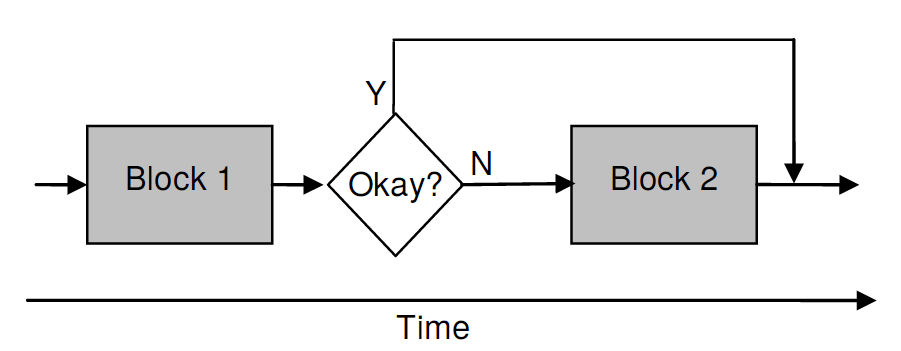
\includegraphics[scale=0.3]{grafiken/recovery-block.png}		
		\caption{Ansatz der Recovery-Blocks
			\footnotemark		
		}		
	\end{figure}
	\footnotetext{Quelle: \cite{lucent}}
\end{frame}
%
%
\begin{frame}
	\frametitle{Ansätze für zuverlässige Systeme - Recovery Blocks (2)}
	Eigenschaften:
	\begin{itemize}
		\item Akzeptanztest kann so aufwendig wie die eigentliche Funktionalität werden
		\item Zeitliche Verzögerung im Falle eines fehlgeschlagenen Tests
	\end{itemize}	
\end{frame}
\section{N-Version Programmierung}
\subsection{Definition}
%
%
\begin{frame}
	\frametitle{Überblick}
	\tableofcontents[currentsubsection]
\end{frame}
%
%
\begin{frame}
	\frametitle{N-Version Programmierung - Definition}
	\begin{block}{Definition: N-Version Programmierung \cite{Chen1978}}
		\enquote{\emph{N-version programming is defined as the independent generation of $ N \geq 2 $ functionally equivalent programs, called \enquote{versions}, from the same initial specification.}}
	\end{block}
\end{frame}
%
\subsection{Konzepte}
%
%
\begin{frame}
	\frametitle{Überblick}
	\tableofcontents[currentsubsection]
\end{frame}
%
%
\begin{frame}
	\frametitle{N-Version Programmierung - Konzepte (1)}
	Nebenläufige Berechnung der Ergebnisse der N-Versionen:
	\begin{figure}
		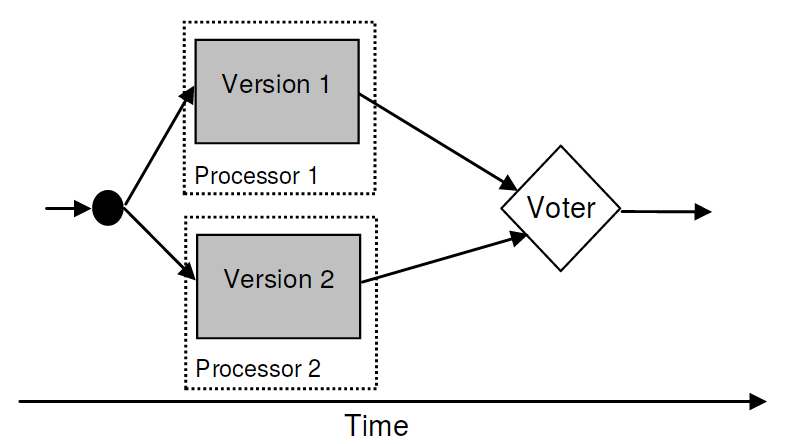
\includegraphics[scale=0.3]{grafiken/multi-thread-n-version.png}		
		\caption{N-Version Software-Unit im Falle von Multi-Threading
			\footnotemark		
		}		
	\end{figure}
	\footnotetext{Quelle: \cite{lucent}}
\end{frame}
%
%
\begin{frame}
	\frametitle{N-Version Programmierung - Konzepte (2)}
	Besondere Komponenten einer N-Version Software-Unit
	\begin{itemize}
		\item Vergleichsvektoren
		\begin{itemize}
			\item Zustand der jeweiligen Version
			\item Variablen, Ereignisse...
		\end{itemize}
		\pause
		\item Vergleichsindikatoren
		\begin{itemize}
			\item Ausgang eines Vergleichs
			\item Anzustoßende Aktion
		\end{itemize}
		\pause
		\item Synchronisationsmechanismen
		\begin{itemize}
			\item Signale zwischen Versionen und Treiber
		\end{itemize}
	\end{itemize}
\end{frame}
%
%
\begin{frame}
	\frametitle{N-Version Programmierung - Konzepte (3)}
	Aufstellen der gemeinsamen Spezifikation:
	\begin{itemize}
		\item Zu implementierende Funktion
		\item Datenformat der Vergleichsvektoren
		\item Zu verwendende Vergleichsalgorithmus
		\item Auf Ausgänge der Vergleiche folgende Aktionen
	\end{itemize}
\end{frame}
%
%
\subsection{Beispiele}
%

\section{Experimente}
%
\subsection{Wahl der Spezifikationssprache}
%
%
\begin{frame}
	\frametitle{Überblick}
	\tableofcontents[currentsubsection]
\end{frame}
%
\begin{frame}
	\frametitle{Wahl der Spezifikationssprache (1)}
	Experiment von 1978-1983 \cite{Avizienis:1984:FTD:1319725.1320045}:
	\begin{itemize}
		\item Szenario: Flughafenverwaltung
		\item Spezifikation in OBJ, PDL und Englisch geschrieben
		\item 18 Versionen in PL/1 implementiert
		\item 7 OBJ, 5 PDL und 6 englische Versionen
		\item PDL-Spezifikation mit 74 Seiten vs. 13 bei der OBJ- und 10 bei der englischen Spezifikation
	\end{itemize}
	
\end{frame}
%
%
\begin{frame}
	\frametitle{Wahl der Spezifikationssprache (2)}
	Durchführung des Experiments mit 100 Testtransaktionen:
	\begin{itemize}
		\item Transaktionsendpunkte als Vergleichsstellen
		\item 18-facher Vergleichsalgorithmus zur Ermittlung der korrekten Ergebnisse
		\item 816 Tripel-Kombinationen der Versionen getestet
	\end{itemize}	
\end{frame}
%
%
\begin{frame}
	\frametitle{Wahl der Spezifikationssprache (3)}
	Beobachtungen:
	\begin{itemize}
	\item Reine PDL-Tripel leicht zuverlässiger
	\item Jedoch kein gravierender Unterschied bezüglich der Spezifikationssprachen
	\item Mangelnde Präzision und Ausdrucksmöglichkeiten der untersuchten Sprachen
	\item Fehlinterpretationen der Spezifikationen
	\item Unabhängige Fehlerursachen führten häufig zu den selben falschen Ergebnissen.
	\end{itemize}	
\end{frame}
%
%
\subsection{Unabhängigkeit der Fehler}
%
\begin{frame}
	\frametitle{Überblick}
	\tableofcontents[currentsubsection]
\end{frame}
%
\begin{frame}
	\frametitle{Unabhängigkeit der Fehler}
	\begin{itemize}
		\item Annahme der N-Version Programmierung:
			\begin{itemize}
				\item Unabhängige Entwicklungskonditionen führen zu unabhängigen Fehlern in den einzelnen Versionen.
				\item Verschiedene Versionen versagen unabhängig voneinander.
				\item Zuverlässigkeit des Gesamtsystems ist deutlich höher als die der einzelnen Versionen.
			\end{itemize}
			\pause
			\item Aber:
			\begin{itemize}
				\item Programmierer tendieren bei anspruchsvollen Aufgaben dazu die selben Fehler zu machen.
				\item Enorme zusätzliche Kosten in der Entwicklung multipler Versionen
				\item Lohnt sich der Aufwand?
				\item $\implies$ Annahme der Fehlerunabhängigkeit untersuchen
			\end{itemize}
		
	\end{itemize}
	
\end{frame}
%
%
\begin{frame}
	\frametitle{Knight \& Leveson Experiment (1)}

	 Experiment zur Überprüfung der Unabhängigkeit von Fehlern in Versionen \cite{Knight:1986:EEA:10677.10688}:
		\begin{itemize}
			\item Raketenabwehrsystem als Zielprogramm
			\item Doktoranden und Studenten der University of Virginia und der University of California
			\item 27 Versionen in Pascal auf Basis einer Spezifikation
			\item 241 Bit Vergleichsvektoren
			\item 1 Millionen automatisch generierte Testfälle
			\item Existierendes \enquote{\emph{Goldprogramm}} als Vergleichsmaßstab
			
		\end{itemize}

\end{frame}
%
%
\begin{frame}
	\frametitle{ Knight \& Leveson Experiment(2)}
	
	Ergebnisse:
	\begin{itemize}
		\item Hohe Zuverlässigkeit in allen Versionen ($\geq 99\%$)
		\item Trotzdem hohes Auftreten gemeinsamer Fehler in Testfällen
		\item In 1255 Fällen versagte mehr als eine Version
		\item In 2 Fällen versagten sogar 8 Versionen
		\item Mehr gemeinsame Fehler aufgetreten, als bei eine Normalverteilung von unabhängigen Fehlern anzunehmen wäre
		\item Fehler aufgrund von mangelhaften mathematischen Kenntnissen
		\item Annahme der Fehlerunabhängigkeit zurückgewiesen		
	\end{itemize}
	\pause
	
	Auf die nachfolgende Kritik des Experiments reagierten Knight und Leveson mit einer umfangreichen Antwort \cite{reply_critics}.
	
\end{frame}

\subsection{Aktuelle Forschungsprojekte}
%
%
\begin{frame}
	\frametitle{Überblick}
	\tableofcontents[currentsubsection]
\end{frame}
%
\begin{frame}
	\frametitle{Aktuelle Forschungsprojekte}
	
	\center{\huge{Wie geht's weiter?}}
	
\end{frame}
%
%
\begin{frame}
	\frametitle{N-Version Website}
	
	\begin{itemize}
		\item 3 Versionen eines Online-Auktionshauses \cite{zero-day}
		\item Unterschiede in den Komponenten:
		\begin{itemize}
			\item Betriebssystem
			\item Webserver
			\item Programmiersprache
			\item DBMS
		\end{itemize}
		\item Ziel: Robustheit gegenüber Zero-Day-Exploits
		\item Schwachstelle: Verwaltender HTTP-Dispatcher
		
	\end{itemize}
	
\end{frame}
%
%
\begin{frame}
	\frametitle{Cloud-basierte Antiviren-Software}
	
	CloudAV, Antiviren-System als Netzwerk-Service in der Cloud \cite{Oberheide:2008:CNA:1496711.1496718}: 
	\begin{itemize}
		\item 10 verschiedene Viren-Erkennungssysteme
		\item $35\%$ höhere Erkennungsrate als herkömmliche Systeme bei aktuellen Gefahren
	\end{itemize}
	\pause
	\begin{figure}
		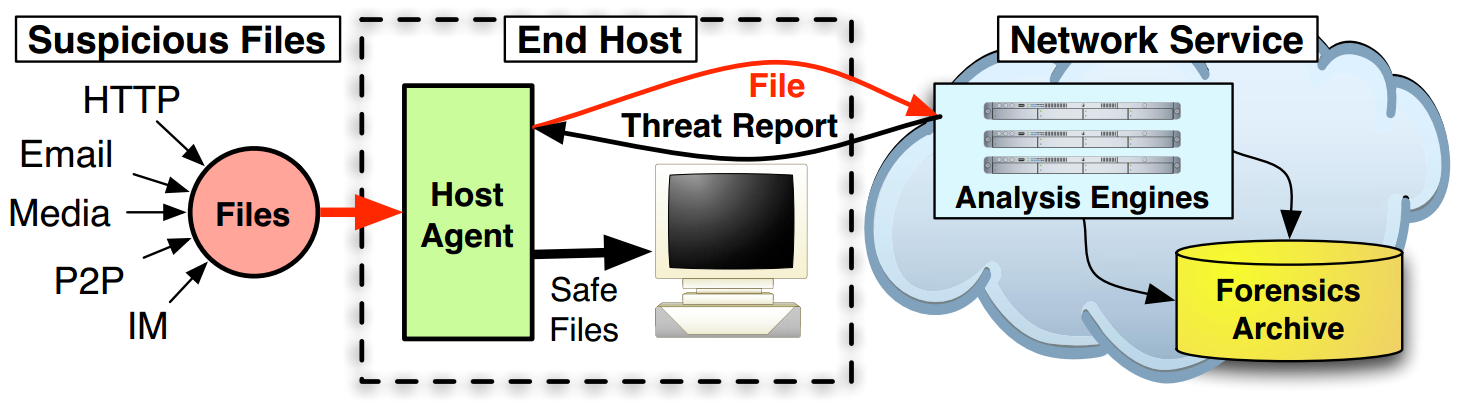
\includegraphics[scale=0.2]{grafiken/antivir.png}		
		\caption{Konzept CloudAV
			\footnotemark		
		}		
	\end{figure}
	\footnotetext{Quelle: \cite{Oberheide:2008:CNA:1496711.1496718}}
\end{frame}
%

\section{Fazit}
\begin{frame}
	\frametitle{Überblick}
	\tableofcontents[currentsection]
\end{frame}
%
\begin{frame}
	\frametitle{Fazit - Beobachtungen}

	\begin{itemize}
		\item N-Version Programmierung ermöglicht Fehlertoleranz eines Software-Systems durch funktionelle Redundanz
		\item Erhöhte Kosten durch Entwicklung mehrerer Versionen
		\item Potentiell niedrigere Kosten durch geringeren Testaufwand
		\item Unabhängigkeit der Fehler in Frage gestellt
		\item Einsatzbeispiele vor allem in der Luftfahrt
	\end{itemize}
\end{frame}
%
%
\begin{frame}
	\frametitle{Fazit - Ausblick}
	
	\begin{itemize}
		\item Neue Einsatzmöglichkeiten im Bereich Webservices
		\item Neues Ziel der Robustheit gegen böswillige Angriffe
		\item Kommunikationsverbot zwischen Entwicklerteams lockern
		\item Benötigte Kenntnisse der Programmierer überprüfen
	\end{itemize}
\end{frame}
%
%\input{literatur.tex}

\begin{frame}[allowframebreaks]
	\frametitle{Literatur}
	\bibliographystyle{apalike}
	\bibliography{literatur}
\end{frame}

%\input{example.tex}


\end{document} 